\documentclass[11pt,a4paper]{article}
\usepackage[hyperref]{acl2018}
\usepackage{times}
\usepackage{latexsym}
\usepackage{graphicx}
\usepackage{url}

\aclfinalcopy % Uncomment this line for the final submission
%\def\aclpaperid{***} %  Enter the acl Paper ID here

%\setlength\titlebox{5cm}
% You can expand the titlebox if you need extra space
% to show all the authors. Please do not make the titlebox
% smaller than 5cm (the original size); we will check this
% in the camera-ready version and ask you to change it back.

\newcommand\BibTeX{B{\sc ib}\TeX}

\title{Optimization Method Coding Project 3: \\ Non-linear Least Square Problems}

\author{Li, Ziyao \\
  1500017776 / Yuanpei College \\
  {\tt leeeezy@pku.edu.cn}
  }

\date{}

\begin{document}
\maketitle
\begin{abstract}
  This work focuses on methods solving non-linear least square problems. Six test functions are evaluated in this work, namely Meyer Function, Osborne Exponential I Function, Osborne Exponential II Function, Jennrich and Sampson Funtion, Freudenstein and Roth Function and Davidon Function. Numerical Experiments are conducted on three formerly mentioned problems. Six methods are examined with these problems. Generally Gauss-Newton (GN) method have higher convergence speed, while the exact line search used in it adds greatly to its function-evaluation times. Levenberg-Marquardt-Fletcher (LMF) method and Levenberg-Marquardt-Nielson (LMN) method show similar performances. Dogleg and Twofold Dogleg methods do not perform well on the problem. Gauss-Newton method with the BFGS adjustment for Large-Residual problem is the most robust method with more iterations to converge in different problems.
\end{abstract}

\section{Least Square Problem}

Least Square Problems are defined as
\begin{displaymath}
  \min_x f(x) = \sum_{i=1}^{m}r_i(x).
\end{displaymath}
This kind of problems are special because the gradients of the problem can be transformed to
\begin{displaymath}
  g(x) = J'(x)r(x),
\end{displaymath}
and approximations over the Hesse matrices of original problems can be made by calculating the Jacobian matrices, and Newton directions can be estimated over the Gauss-Newton equation
\begin{displaymath}
  J'_k J_k d_k = -J'_k r_k.
\end{displaymath}

Levenberg-Marquardt methods adjust the matrix $J'_k J_k$ into $J'_k J_k + \nu_k I_n$ to avoid problems caused by the singularity of the original matrix; Dogleg methods adopt the idea of Trust Region Algorithms when deriving the descend directions and step-lengths by combining the Gauss-Newton direction and negative gradient direction; for problems with large residuals, ignoring the matrix $S(x)$ can cause problems, and BFGS methods can be used to calculate the $B(x)$ matrices to approximate $S(x)$, leading to robustness and faster convergence.

\section{Numerical Performance}

Performance of six different methods are tested. The general convergence criterion, without specific notifications, are defined as
\begin{eqnarray*}
  |f_{k} - f_{k-1}| & \le & \epsilon \\
  ||g_{k}||_{\infty} & \le & \epsilon \\
  \epsilon & = & 10^{-8}.
\end{eqnarray*}
However, due to the property of some of the problems, $g_k$ hardly converges to $10^{-8}$ no matter what method is used. Therefore, an alternative criterion without constraints over $g_k$ is used sometimes and the factor indicating performance, $\Vert g_k \Vert_{\infty} / \Vert g_0 \Vert_{\infty}$, is monitored when such criterion is used. Relevant results are shown in Table 1.

\begin{table*}
\label{tab3}
\centering
\begin{tabular}{l}
\begin{tabular}{l|rrr|rrr|rrr}
\hline
 &
\multicolumn{3}{|c}{\textbf{GN}} &
\multicolumn{3}{c}{\textbf{LMF}} &
\multicolumn{3}{c}{\textbf{LMN}} \\
\hline
Problem &
iter & feva & $g$ &
iter & feva & $g$ &
iter & feva & $g$ \\
\hline
Meyer & *8 & 350 & 10 & *160 & 321 & 13 & *495 & 991 & 10 \\
Osborne I & 10 & 442 & - & 27 & 55 & - & 22 & 45 & - \\
Osborne II & 13 & 570 & - & 19 & 39 & - & 14 & 29 & - \\
Jennrich and Sampson & / & / & / & 91 & 183 & - & 159 & 319 & - \\
Freudenstein and Roth & 41 & 1,892 & - & 51 & 103 & - & *32 & 65 & 6 \\
Davidon & *625 & 29,375 & 7 & *75 & 151 & 9 & *77 & 155 & 8 \\
\hline
 &
\multicolumn{3}{|c}{\textbf{Dogleg}} & \multicolumn{3}{c}{\textbf{Twofold-Dogleg}} & \multicolumn{3}{c}{\textbf{GN+BFGS}} \\
\hline
Problem &
iter & feva & $g$ &
iter & feva & $g$ &
iter & feva & $g$ \\
\hline
Meyer & *95 & 154 & 11 & *86 & 150 & 14 & *110 & 7,603 & 9 \\
Osborne I & 9 & 17 & - & 18 & 32 & - & 22 & 1,243 & - \\
Osborne II & 13 & 26 & - & 18 & 33 & - & 27 & 1,493 & - \\
Jennrich and Sampson & *27 & 40 & 8 & *38 & 58 & 7 & 8 & 656 & - \\
Freudenstein and Roth & 41 & 66 & - & *31 & 49 & 7 & 7 & 306 & - \\
Davidon & *255 & 455 & 7 & *100 & 176 & 7 & 13 & 991 & - \\
\hline
\end{tabular} \\
\begin{tabular}{l}
  /: Algorithm cannot continue. \\
  $*$: Criterion without constraining $g$ adopted. \\
  $g$: $-lg(\frac{\Vert g_k \Vert_{\infty}}{\Vert g_0 \Vert_{\infty}})$, calculated if * is adopted.
\end{tabular}
\end{tabular}
\caption{Numerical performance of six methods over six problems. The functions can be found in \textit{Testing Unconstrained Optimization Software}, or relevant references attached to this report.}
\end{table*}

Due to the calculation of exponential, sine and cosine functions, the computational accuracy in this projects are relatively low, causing much trouble when line search methods are adopted. Figure 1 shows the function values versus step lengths of the Meyer Function, from which we can see obvious fluctuations caused by machine accuracy. Therefore, if valid step lengths cannot be derived, we set $\alpha=1$ instead of speculating that the direction is non-descending and exiting, as we may do in the Quasi-Newton Methods.

\begin{figure}[ht]
\vskip 0.2in
\label{fig1}
\begin{center}
\centerline{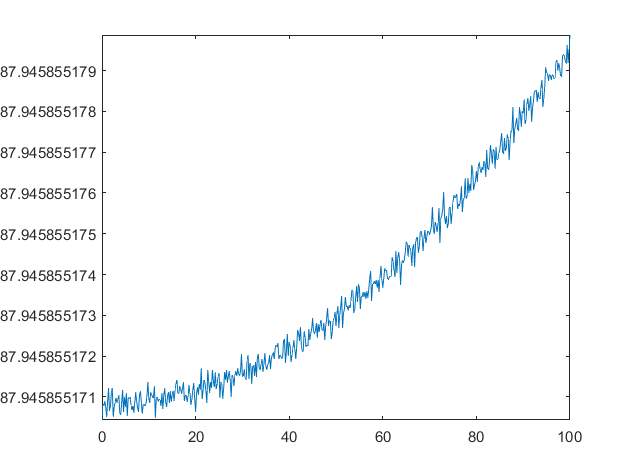
\includegraphics[width=\columnwidth]{fig1}}
\caption{A Figure of function value versus step length during some iteration of the Meyer Function. The function suffers from giant fluctuations caused by limited machine accuracy, which is mainly caused by the exponential operation in the Meyer Function.}
\end{center}
\vskip -0.2in
\end{figure}

The gradient of Meyer function never reaches a level below $10^{-5}$. This is mainly caused by the exponential part of the function, evaluation errors and small denominators ($x_3$). GN method behaves surprisingly good over this problem, while it cannot continue at iteration $9$. Other methods all have poor performance over this problem.

The Osborne Exponential problems have rather good numerical properties. Although the dimensionality of the problem is the most during all six problems, they still remain the two easiest problems. All methods show good performances over these problems, among which the Dogleg method's is the best.

Surprisingly, the methods targeting at small residual problems are able to solve large residual problems as well, while the gradient usually do not converge in reasonable iterations, and the performances are poor. GN+BFGS performs extremely good over these three problems, while the function-evaluation times are massive due to the exact line search process.

\section{\texttt{lsqnonlin()} Performance}

\texttt{lsqnonlin()} is an inner function defined in Matlab. We examined the performance of this function over these six problems, finding that processes terminate with different reasons. For Meyer, Osborne Exponential II and Freudenstein \& Roth functions, the iterations stop because function values stop changing ($g$ not converged). For Osborne Exponential II function, both function value and $g$ converge. For Jennrich \& Sampson function, the step length is so small to continue. For Davidon function, the iteration maximun ($400$) reached. Besides, for Freudenstein \& Roth function, the local minimum is obtained.
\end{document}
